\documentclass{article}
\usepackage[a4paper, total={6.5in, 9in}]{geometry}
\usepackage{amsmath}
\usepackage{amssymb}
\usepackage{graphicx}
\usepackage{subfigure}
\usepackage{hyperref}
\usepackage{booktabs}
\usepackage{authblk}
\usepackage{float}
\renewcommand{\labelenumi}{(\alph{enumi})}
\title{CSCI-SHU 360 Machine Learning\\
    Solution to homework 3}
\author{Josiah Li \texttt{yl11912@nyu.edu}}

\begin{document}
    \maketitle
\section{Programming Problem: Logistic Regression}
\subsection{}
By extended representation, we have $ X\gets [X,1] \in \mathbb{R}^{n\times (d+1)} $, and $ W\gets [W, b]\in \mathbb{R}^{(d+1)\times c} $. For $X_i$, we have $ z_i=X_iW $. And we have $ Pr(y=k|x=X_i;W) = \dfrac{\exp{(z_k)}}{\sum_{j=1 }^{c } \exp{(z_j)}}  = P_{i,k}$\\ 
For the loss function $ F(x) $, we have: 
\begin{align*}
    F(x) &= \frac{1}{n} \sum_{i=1}^{n} -\log[Pr(y=y_i|x=X_i;W)] + \frac{\eta}{2}\Vert W\Vert ^2_F\\ 
         &= \frac{1}{n} (\sum_{i=1}^{n} -(z_{y_i}) + \sum_{i = 1}^{n}\log{\sum_{j=1 }^{c } \exp{z_j}} )+ \frac{\eta}{2}\Vert W\Vert ^2_F\\ 
         &= \frac{1}{n} (-\sum_{i=1}^{n} X_{i}W_{:,y_i} + \sum_{i=1}^{n} \log \sum_{j=1 }^{c } \exp{X_iW_{:,j}}) + \frac{\eta}{2}\Vert  W\Vert ^2_F\\
         &= \frac{1}{n} (-\sum_{i=1}^{n} X_{i}W_{:,y_i} + \sum_{i=1}^{n} \log \sum_{j=1 }^{c } \exp{X_iW_{:,j}}) + \frac{\eta}{2}\sum_{j=1 }^{c} \Vert  W_{:,j}\Vert ^2_F
\end{align*}
Thus we take the partial derivative:
\begin{align*}
    \frac{\partial F(X)}{\partial W_j} &= \frac{1}{n} (-\sum_{i=1}^{n} \mathbf{1}\{y_i = j\}X_i^T + \sum_{i=1}^{n} \frac{\exp{(X_iW_j)}X_i^T}{\sum_{k=1 }^{c } \exp{(X_iW_k)}}) + \eta W_j\\
                                       &= \frac{1 }{n}\sum_{i=1}^{n}(P_{i,j} - \mathbf{1}\{y_i = j\})X_i^T + \eta W_j
\end{align*}
If we represent the derivative in numerator layout, we have $ \dfrac{\partial F(W)}{\partial W} = \begin{bmatrix}
\frac{\partial F(W)}{W_1},
\cdots,
\frac{\partial F(W)}{W_c}
\end{bmatrix}$
Let $ \Pi_{i,j} = \mathbf{1}\{y_i = j\}  $, we have:\\
\begin{align*}
    \frac{\partial F(W)}{\partial W} = \frac{1}{n} X^T(P - \Pi) + \eta W
\end{align*}
Thus, after having the gradient of the function, we can have the gradient descent rule for $ W $ which is \begin{align*}
    W\gets W - \lambda (\frac{1}{n}X^T(P-\Pi) + \eta W).
\end{align*}
Where $ \lambda  $ is the learning rate.
\subsection{}
As we know, we have:
\begin{align*}
    \frac{\exp{(a)}}{\exp{(b)}} &= \frac{\exp{(a - c)}}{\exp{(b-c)}}.
\end{align*}
So we have:
\begin{align*}
    \frac{\exp{(z_i)}}{\sum_{j=1}^{c}\exp{(z_j)}} &= \frac{\exp{(z_i - \max\limits_{j}{z_j})}}{\sum_{j=1}^{c}\exp{(z_j - \max\limits_{j}{z_j})}}.
\end{align*}
Which we can see that this modification is the same as origin softmax function.\\ 
Moreover, the original form may lead to an extreme exponential value and lead to a numerical error.\\
We have the following output:\\
\begin{table}[ht]
\centering
\begin{tabular}{|c|c|c|c|c|}
\hline
\textbf{Learning Rate} & \textbf{Converged Iteration} & \textbf{Training Precision} & \textbf{Test Precision} & \textbf{Final Loss} \\
\hline
0.05 & 111 & 0.9829 & 0.9667 & 0.2684 \\
0.005 & 335 & 0.9762 & 0.9644 & 0.1859 \\
0.01 & 219 & 0.9770 & 0.9644 & 0.1795 \\
\hline
\end{tabular}
\caption{Comparison of model performance under different learning rates}
\label{tab:lr_comparison}
\end{table}
\begin{figure}[htpb]
    \begin{center}
        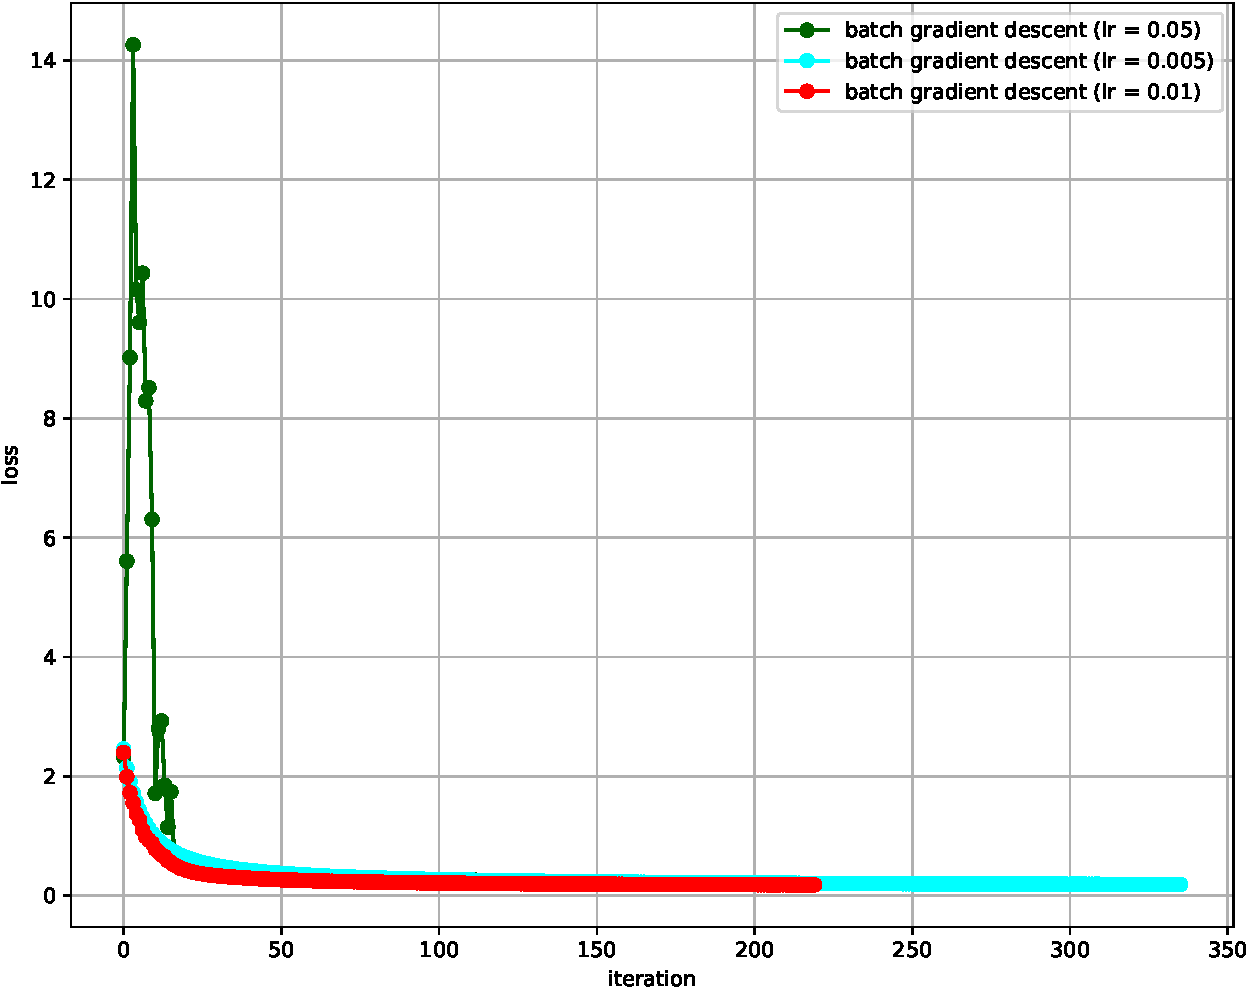
\includegraphics[width=0.5\textwidth]{./figures/logistic_regression_loss.pdf}
    \end{center}
    \caption{Convergence curves under different learning rate.}\label{fig:}
\end{figure}
\subsection{}
As we can see from the graph, for small learning rate, the model is converging in a more stable way but takes more iteration to converge, while the large learning rate will make the convergence less stable, but faster to converge. 
\clearpage
\subsection{}
We have the following output:\\
\begin{table}[ht]
\centering
\begin{tabular}{|c|c|c|c|c|c|}
\hline
\textbf{Learning Rate} & \textbf{Batch Size} & \textbf{Final Epoch} & \textbf{Training Precision} & \textbf{Test Precision} & \textbf{Final Loss} \\
\hline
0.01 & 10  & 21  & 0.996 & 0.971 & 0.4623 \\
0.01 & 50  & 21  & 0.985 & 0.971 & 0.2724 \\
0.01 & 100 & 31  & 0.984 & 0.967 & 0.2590 \\
\hline
0.005 & 10  & 21  & 0.992 & 0.973 & 0.3296 \\
0.005 & 50  & 21  & 0.982 & 0.964 & 0.2491 \\
0.005 & 100 & 26  & 0.972 & 0.960 & 0.2487 \\
\hline
0.001 & 10  & 33  & 0.983 & 0.976 & 0.2538 \\
0.001 & 50  & 58  & 0.975 & 0.956 & 0.2429 \\
0.001 & 100 & 106 & 0.973 & 0.962 & 0.2447 \\
\hline
\end{tabular}
\caption{Performance comparison across different learning rates and batch sizes}
\label{tab:lr_batch_full}
\end{table}
\begin{figure}[htpb]
    \begin{center}
        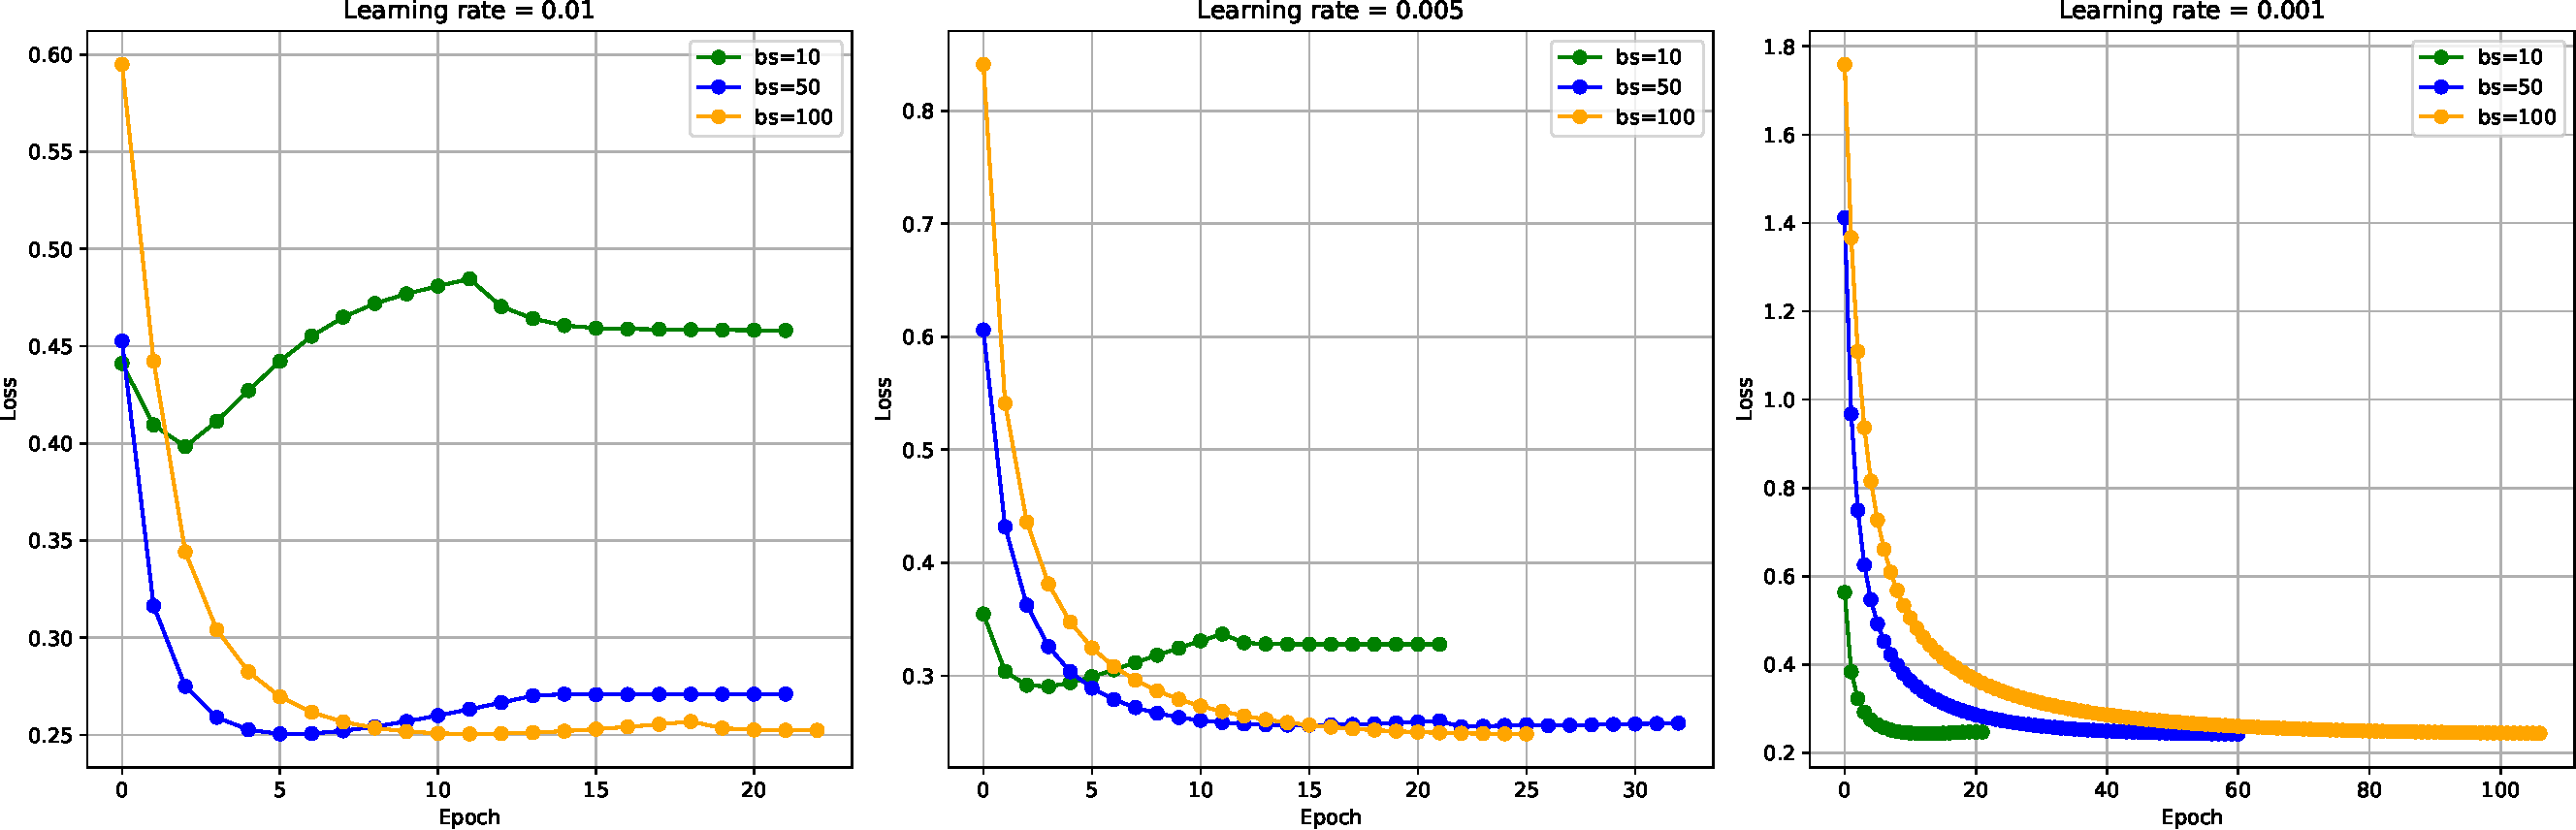
\includegraphics[width=1\textwidth]{./figures/logistic_regression_loss_sgd_subplots.pdf}
    \end{center}
    \caption{Convergence curves under different batch size and learning rate.}\label{fig:}
\end{figure}\\
With the data and figure above, we can see that for the learning rate is small(0.001), the convergence are smooth for all three batch sizes, however, the test precision is generally lower than the other two learning rate settings. And the model takes more time to converge. For the large learning rate(0.01), the model tend to be harder to converge. But under this setting, the $ bs=50 $ and $ bs=100 $ are converging in a much faster speed comparing to the other two learning rate.
\clearpage
\subsection{}
From the previous figure we can see that three batch sizes have different convergence speed with the same initial learning rate. By the instruction from the question, we use $ \frac{10^{-2} \times bs}{100}  $ as the initial learning rate for each batch size $ bs $. The result is:\\ 
\begin{table}[ht]
\centering
\begin{tabular}{|c|c|c|c|c|}
\hline
\textbf{Batch Size} & \textbf{Final Epoch} & \textbf{Training Precision} & \textbf{Test Precision} & \textbf{Final Loss} \\
\hline
10  & 22 & 0.9814 & 0.9689 & 0.2476 \\
50  & 22 & 0.9822 & 0.9733 & 0.2495 \\
100 & 21 & 0.9807 & 0.9711 & 0.2527 \\
\hline
\end{tabular}
\caption{Model performance under different batch sizes with adaptive learning rate}
\label{tab:batch_adaptive}
\end{table}
\begin{figure}[htpb]
    \begin{center}
        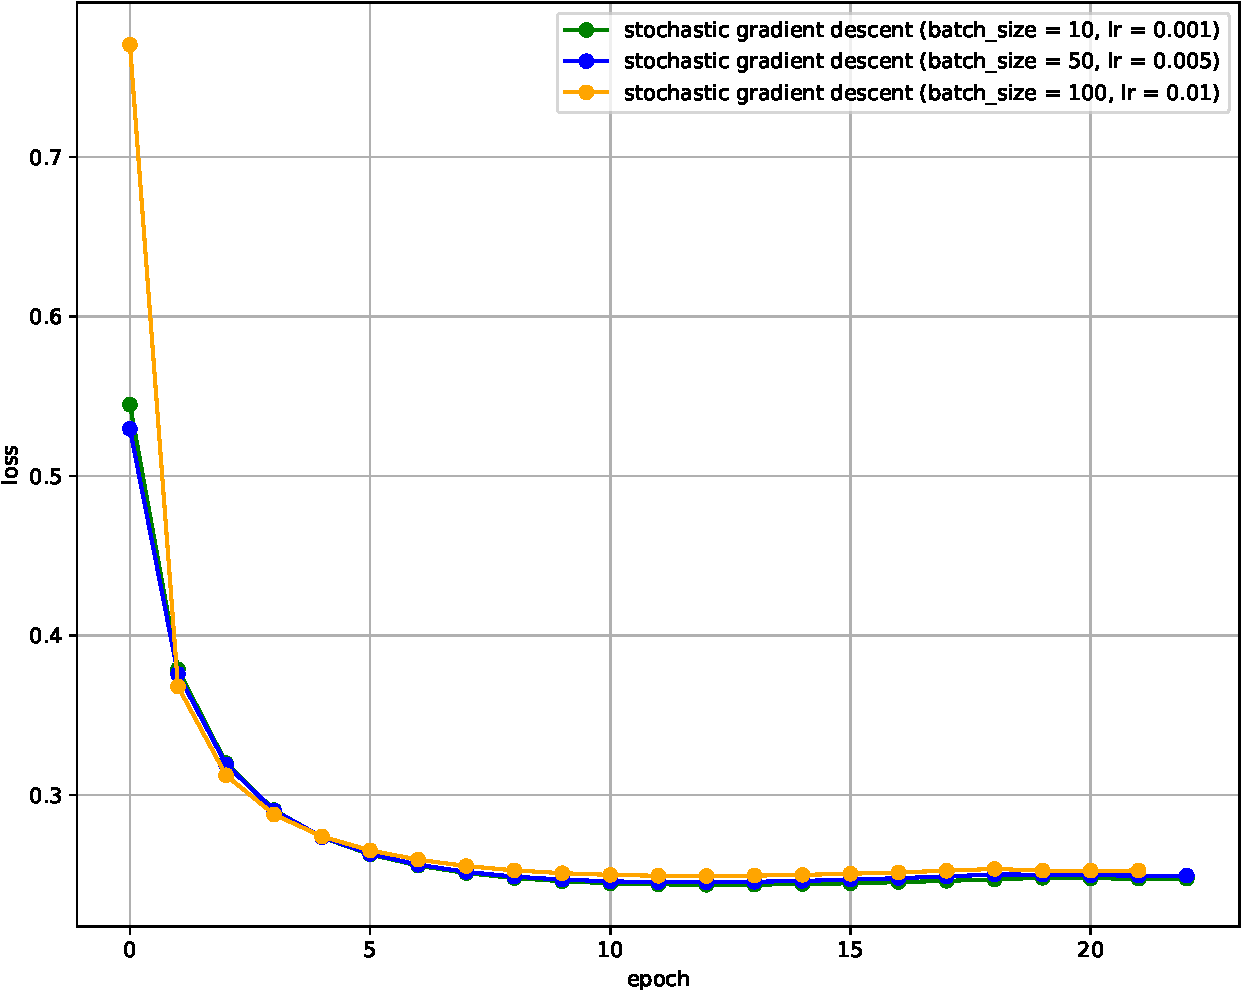
\includegraphics[width=0.75\textwidth]{./figures/logistic_regression_loss_sgd_dynamic.pdf}
    \end{center}
    \caption{Convergence curves by applying different initial learning rate.}\label{fig:}
\end{figure}\\
We can see from the figure that with initial learning rates adjusted according to the batch size, the convergence for all three models became much similar. \\ 
Explanation: when we are doing the SGD, we have $ \Delta W_{epoch} = \dfrac{N}{B} \times \nabla F_{batch}  $. $ N $ is the total number of samples and $ B $ is the batch size. We can see that as $ \nabla_{batch} $ is approximately the general gradient of the dataset. Thus, for every epoch, the smaller batch size leads to larger gradient change per epoch. \\
\clearpage
\section{}
\subsection{}
After performing the coordinate descent, we can have the following curve.
\begin{figure}[htbp]
    \begin{center}
        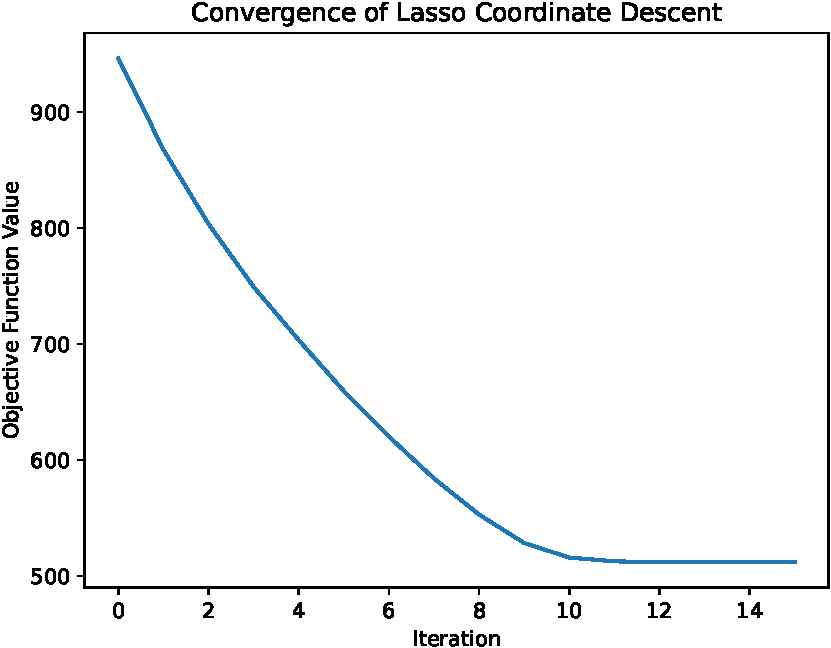
\includegraphics[width=0.5\textwidth]{./figures/lasso_convergence.pdf}
    \end{center}
    \caption{The convergence curve of the Lasso Coordinate Descent.}\label{fig:}
\end{figure}\\ 
The indices of non-zero weight entries are: [ 0,  1,  2,  3,  4, 11, 12, 25, 34, 36, 52, 63, 71].
\subsection{}
We can get the metrics below:\\ 
\begin{table}[ht]
\centering
\begin{tabular}{|c|c|}
\hline
\textbf{Metric}         & \textbf{Value} \\ \hline
RMSE                    & 0.8265       \\ \hline
Sparsity of $w$         & 13           \\ \hline
Precision of $w$        & 0.3846       \\ \hline
Recall of $w$           & 1.0000       \\ \hline
\end{tabular}
\caption{Evaluation Metrics of the Lasso Model}
\label{tab:lasso_eval}
\end{table}
\clearpage
\subsection{}
\begin{figure}[htbp]
    \begin{center}
        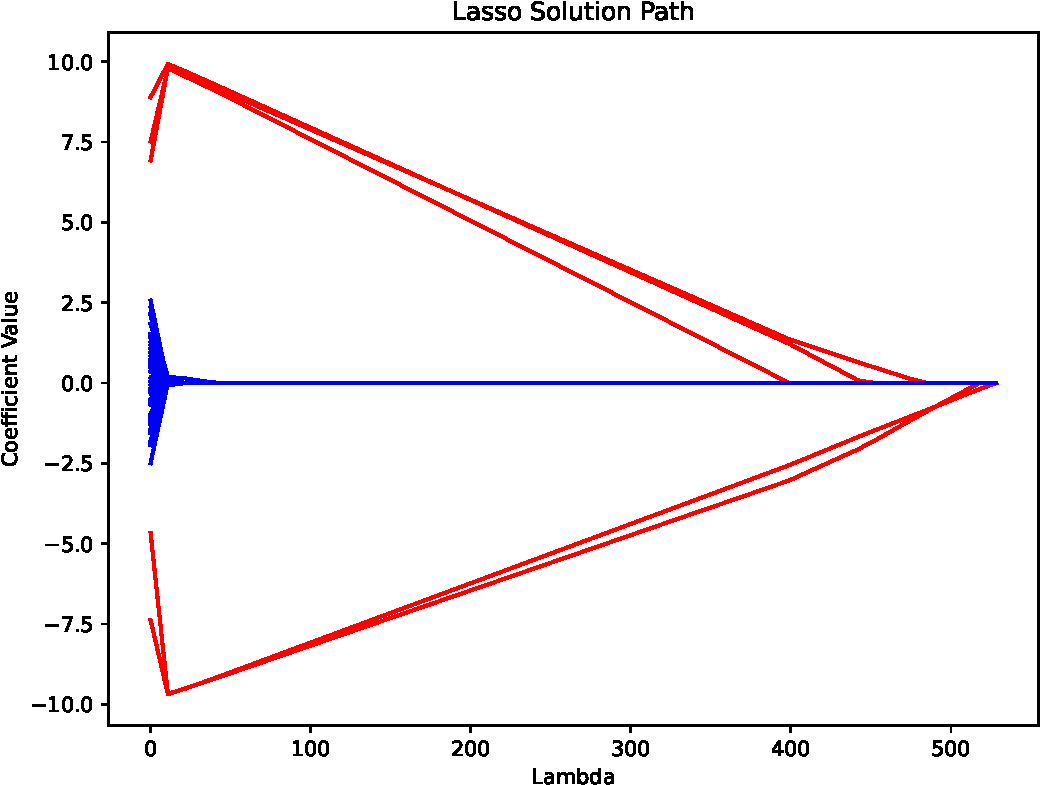
\includegraphics[width=0.5\textwidth]{./figures/lasso_solution_path.pdf}
    \end{center}
    \caption{Lasso solution path for the entries.}\label{fig:}
\end{figure}
From the figure above, we can see that the features are generally saperated into two classes. One class converges to zero in a quick speed while another class will first have a peak before descending. The first class tend to be the zero entries in the real parameters while the other is the non-zero entries in $ \theta $.
\begin{figure}[htbp]
    \begin{center}
        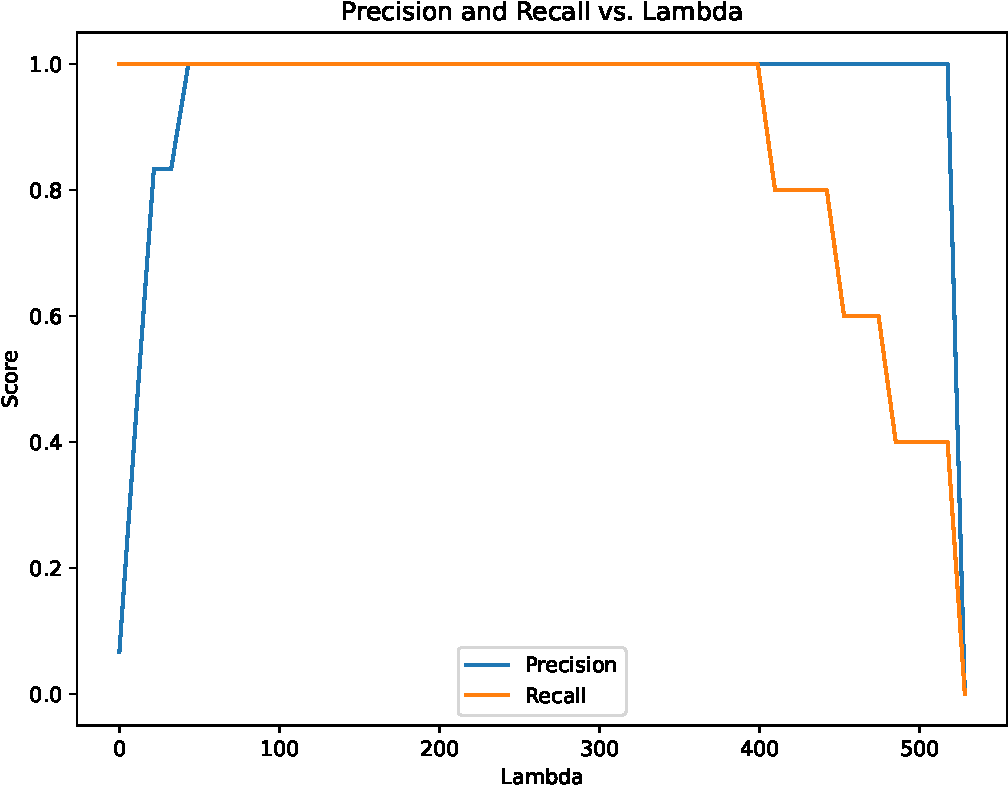
\includegraphics[width=0.5\textwidth]{./figures/lasso_precision_recall_vs_lambda.pdf}
    \end{center}
    \caption{Precision and recall for different $ \lambda $.}\label{fig:}
\end{figure}
From the figure above, we can see that the when we have a large $ \lambda $ the model tend to reduce the scale of $ \theta $ by setting most of the entries to zero. And when we have a smaller $ \lambda $, the model will have less punishment on the scale of the parameters which lead to a high recall rate. Thus, the appropriate $ \lambda $ will pick the valuable entries and abandon the rest.
\clearpage
\begin{figure}[htbp]
    \begin{center}
        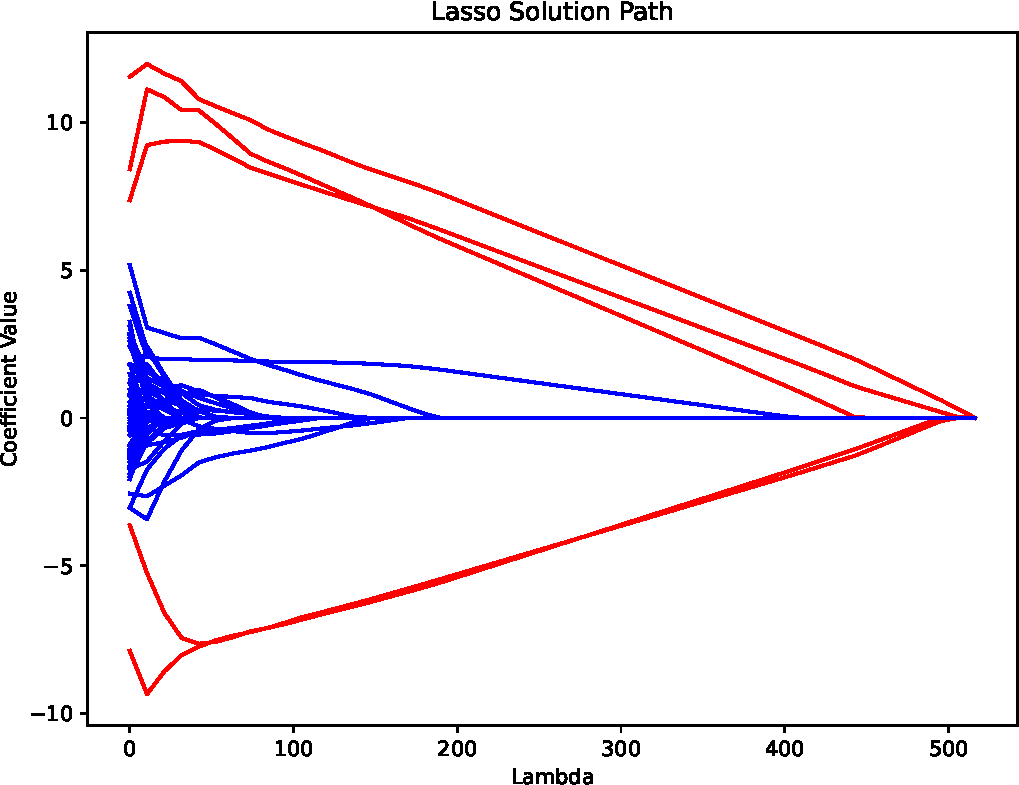
\includegraphics[width=0.5\textwidth]{./figures/lasso_solution_path_large_v.pdf}
    \end{center}
    \caption{Lasso solution path for the entries when $ \sigma = 10 $.}\label{fig:}
\end{figure}
We can see that conparing to the previous figure, with larger $ \sigma $ the convergence of parameters are much more unstable. And as the blue features (the irrelevant features) might have non-zero weight due to the large noise. Under this circumstances, tuning $ \lambda $ become much more important.
\clearpage
\subsection{}
\begin{figure}[htbp]
    \begin{center}
        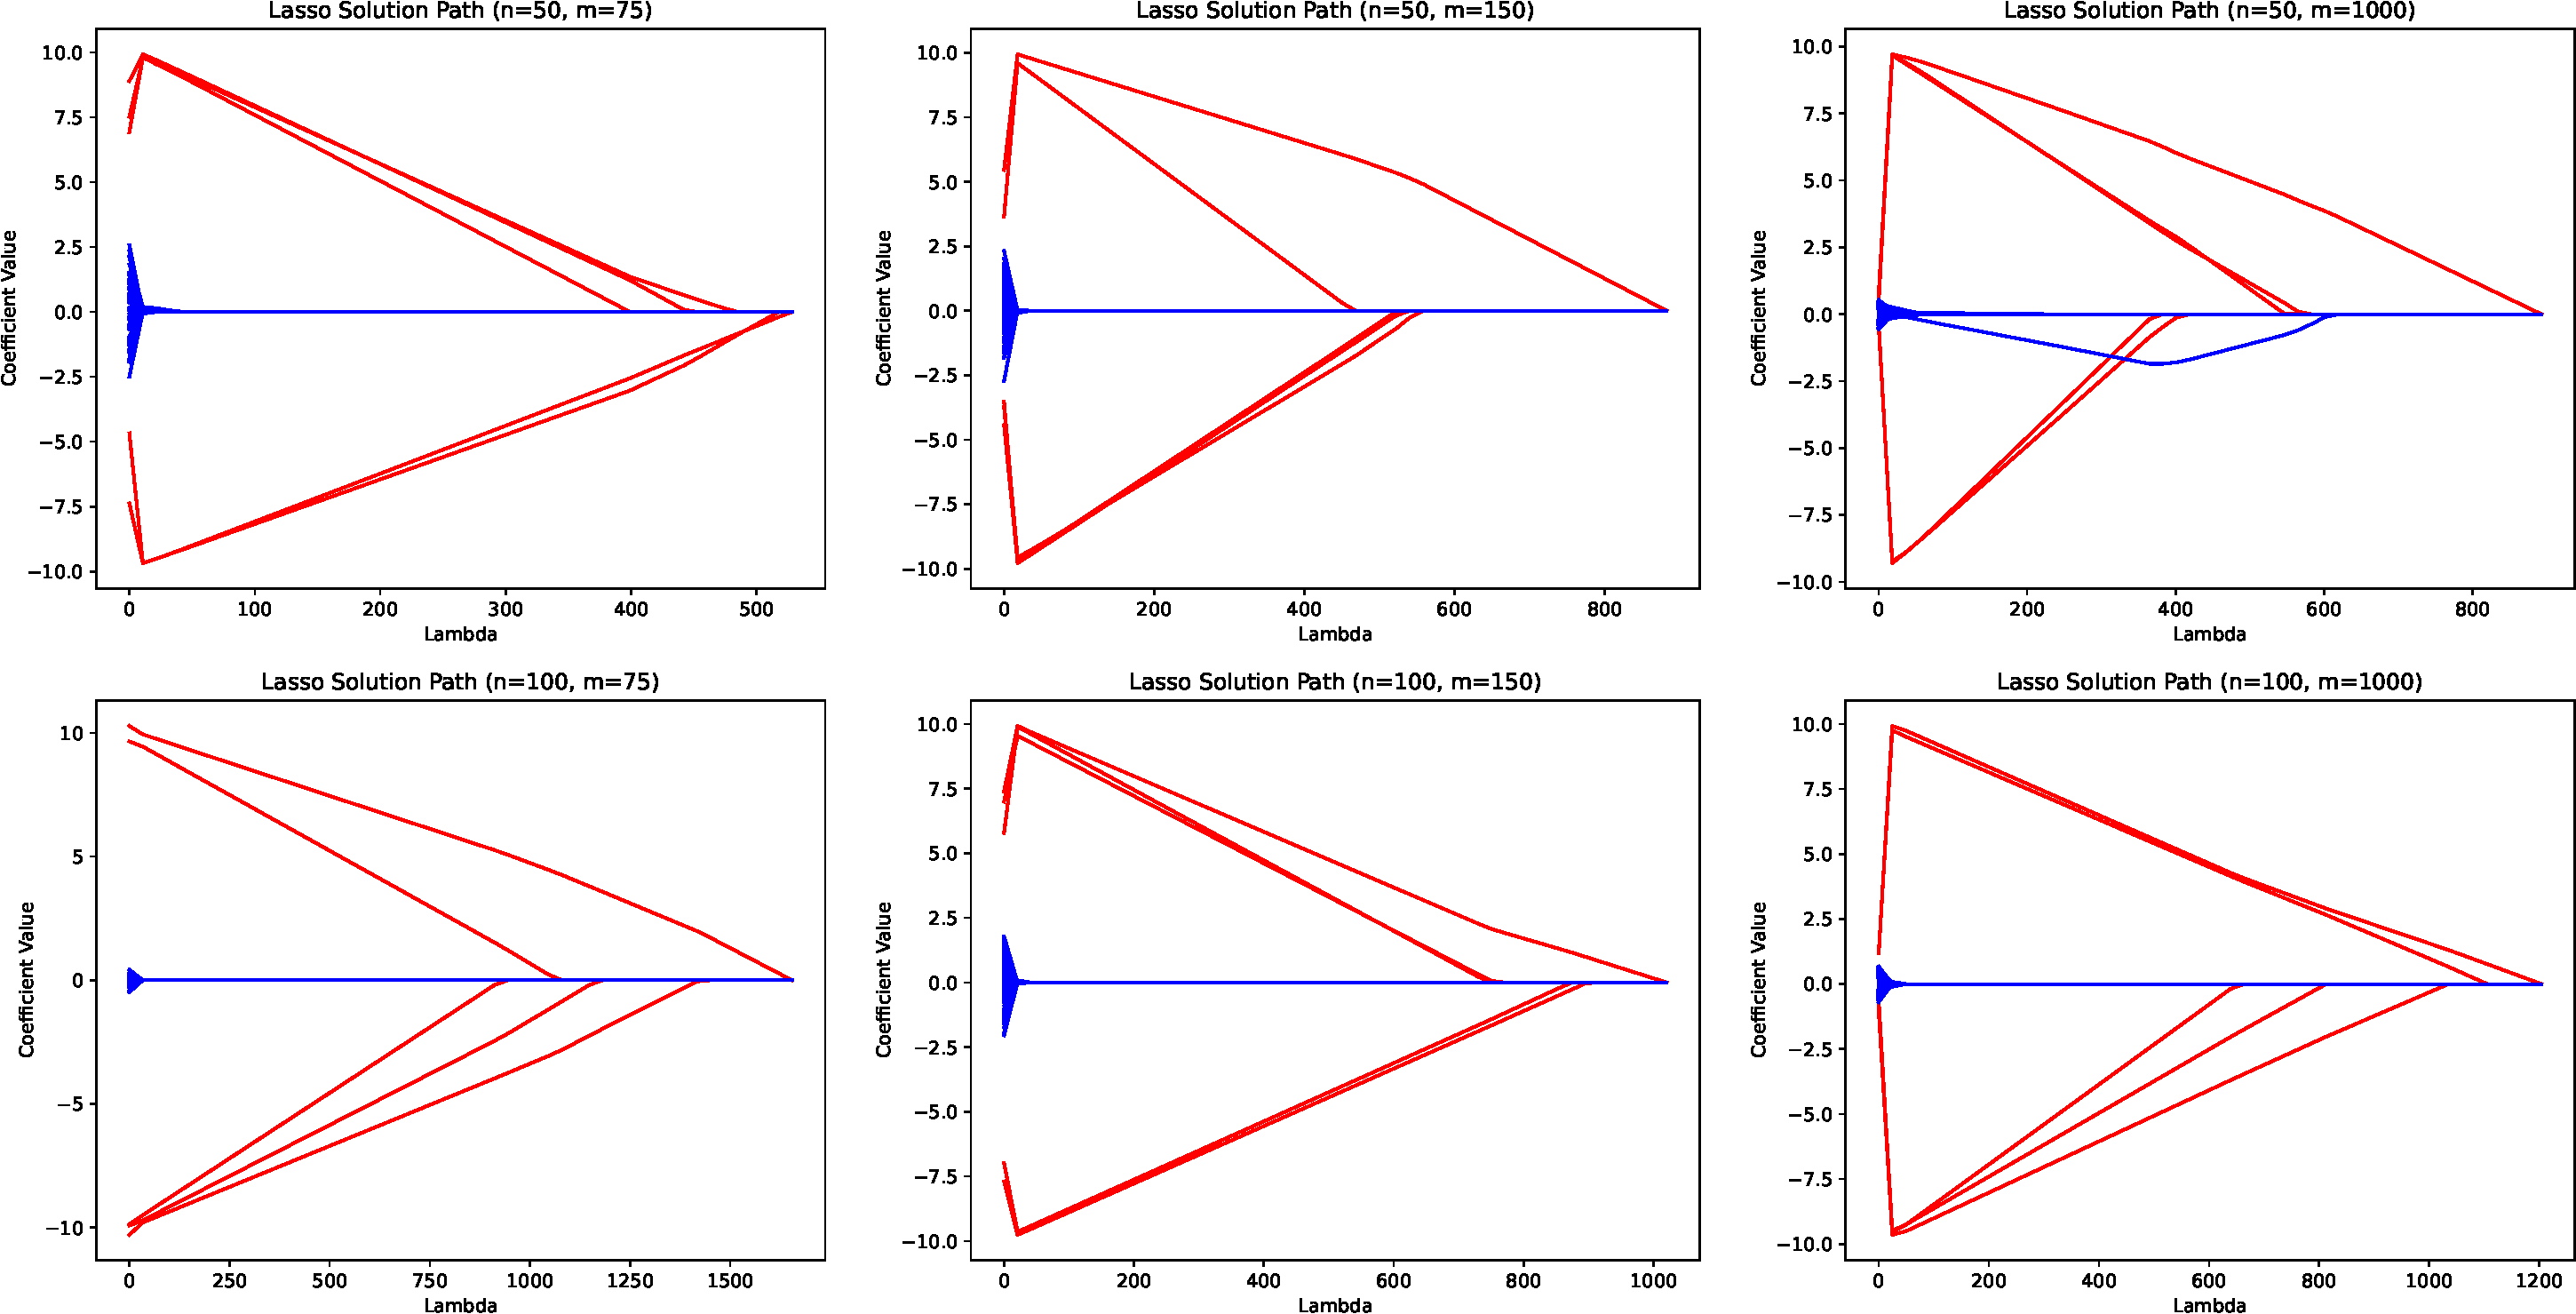
\includegraphics[width=0.85\textwidth]{./figures/lasso_solution_path_n_d_variation.pdf}
    \end{center}
    \caption{The Lasso solution path under different $ n $ and $ m $.}\label{fig:}
\end{figure}
\begin{figure}[htbp]
    \begin{center}
        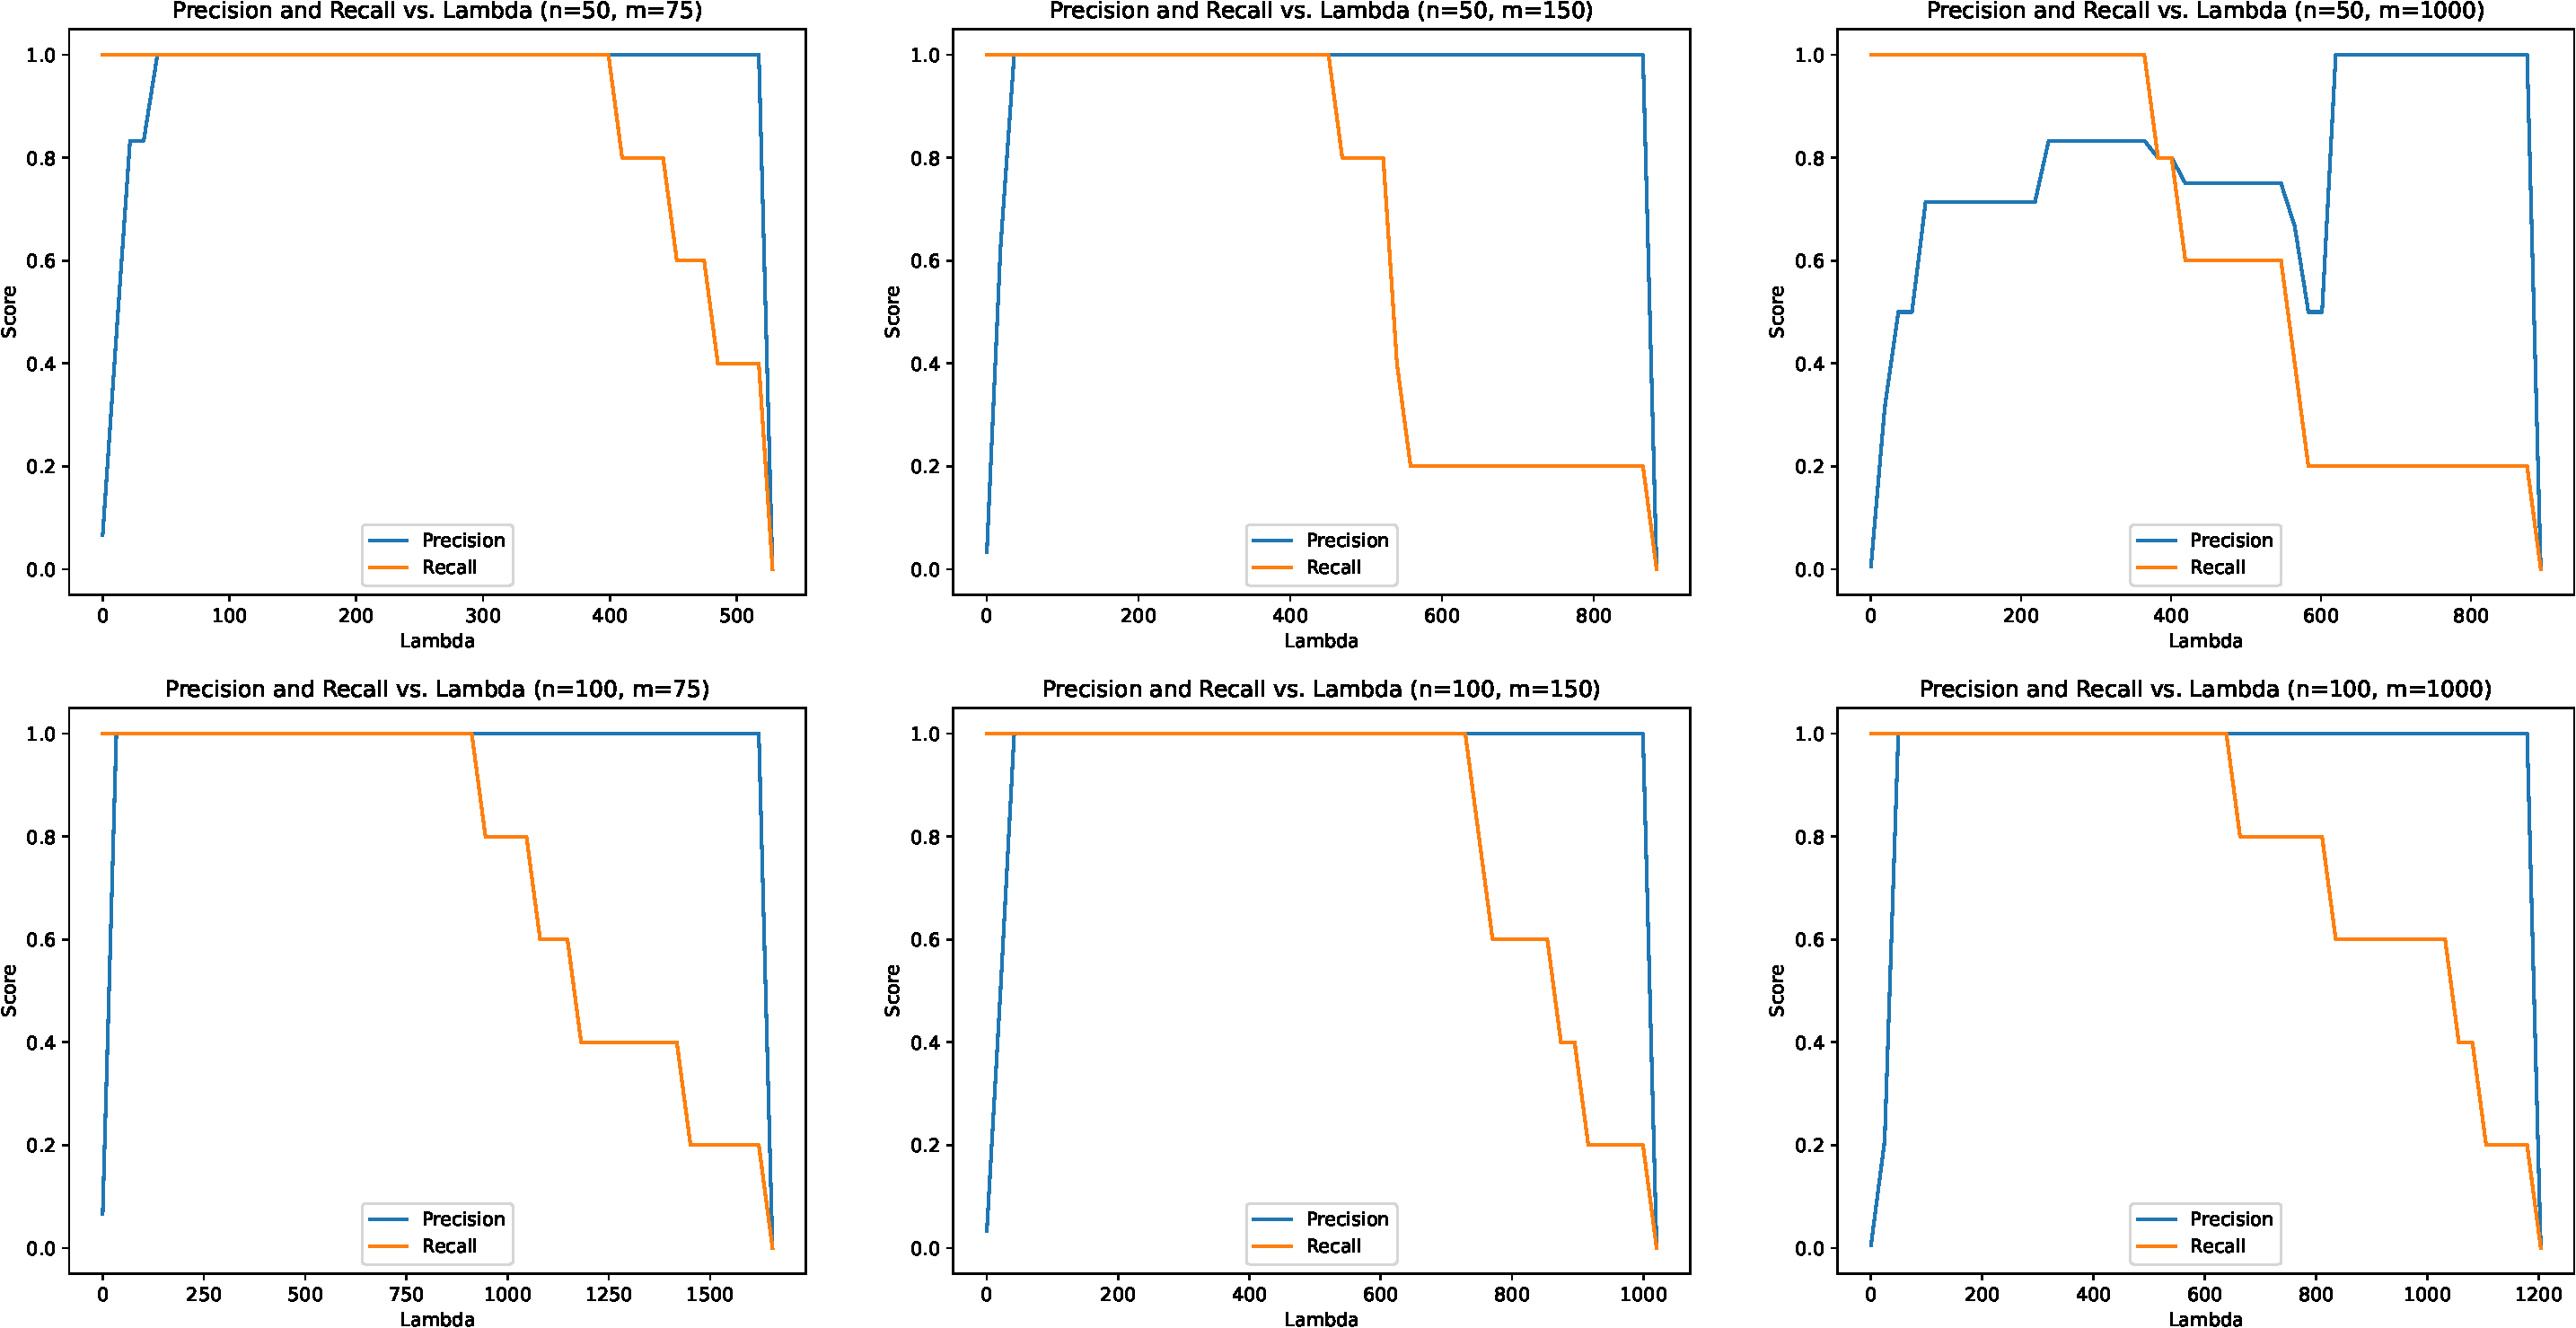
\includegraphics[width=0.85\textwidth]{./figures/eval_precision_recall_vs_lambda.pdf}
    \end{center}
    \caption{The precision and recall under different $ n $ and $ m $.}\label{fig:}
\end{figure}
According to the raw data, we have te table below. To be noted, for $ n=50, m = 1000 $ we are not able to find $ \lambda $ that has both precision and recall to be $ 1 $. Thus, if we have to find a optimal $ \lambda $, by searching for the max sum of precision and recall, it should be $ [236, 365] $(round to integer).
\begin{table}[htbp]
\centering
\caption{The optimal lambda under different $ n $ and $ m $(round to integer).}
\label{tab:optimal_lambda}
\begin{tabular}{c|c|c|c}
\hline
\(n \backslash m\) & 75 & 150 & 1000 \\
\hline
50  & [43, 399] & [36, 450] & [236, 365]$^*$ \\
100 & [34, 911] & [42, 729] & [49, 639] \\
\hline
\end{tabular}
\end{table}
\clearpage
\subsection{}
Implementation: \\
First, the naive implementation was designed for dense matrices and small datasets. And for large and sparse data in Sub-Problem 5, we can use Compressed Sparse Column to optimize the calculation. As csc type is more effcient for column slicing and get non-zero entries in the matrices.\\ 
In the naive implementation, we are calculating the residuals for the $ j $th coordinate by doing an expensive matrix multiplication, which is $ O(n\times m) $ for every coordinate, taking consideration of the total iteration loop $ T $ and number of coordinates, the total time complexity will become $ O(Tnm^2) $. In contrast, if we calculate the residuals outside the inner loop and update the residuals dynamically update the residual matrix. The time complexity for every coordinate will reduce to $ O(n) $, and the total time complexity will reduce to $ O(Tnd) $. Moreover, as we did some small tricks by using csc datatype, we are able to only update the non-zero entries, which reduce the cost in the sparse case.\\

\begin{figure}[htbp]
    \begin{center}
        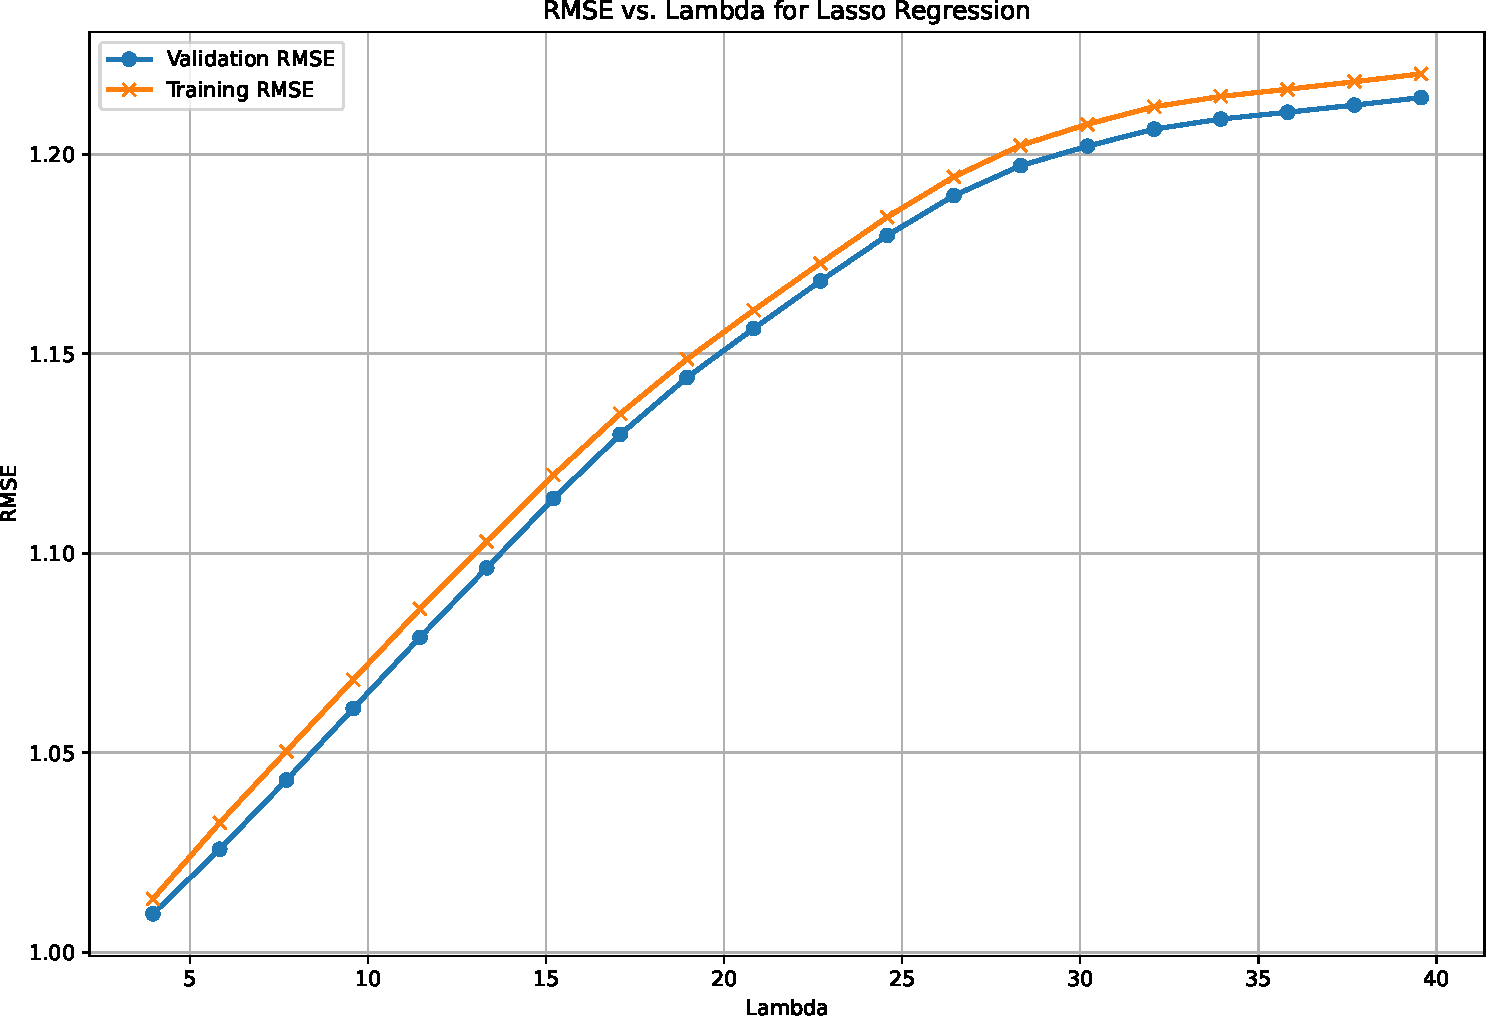
\includegraphics[width=0.9\textwidth]{./figures/lasso_rmse_vs_lambda.pdf}
    \end{center}
    \caption{training and validation rmse v.s. $ \lambda $ values.}\label{fig:}
\end{figure}
\begin{figure}[H]
    \begin{center}
        \includegraphics[width=0.9\textwidth]{./figures/lasso_solution_pathq5.pdf}
    \end{center}
    \caption{the lasso solution path.}\label{fig:}
\end{figure}
\noindent Best lambda: 3.95782540136483 \\ 
Validation rmse: 1.0096512302660232\\
\begin{table}[ht]
\centering
\begin{tabular}{lr}
\hline
\textbf{feature} & \textbf{weight} \\
\hline
great      & 19.626910602812263 \\
not        & -17.746498530426216 \\
best       & 17.05719025532021 \\
amazing    & 14.339641440305963 \\
love       & 12.228556228270259 \\
delicious  & 12.132458330783074 \\
rude       & -11.989863473044203 \\
the worst  & -11.959659903513517 \\
horrible   & -10.486167300825196 \\
awesome    & 10.058457548734463 \\
\hline
\end{tabular}
\caption{top 10 lasso weights.}
\label{tab:lasso_features}
\end{table}

\end{document}
